\documentclass[tikz,border=20pt]{standalone}
\usepackage{tikz}
\usepackage{amsmath}
\usepackage{amssymb}
\usetikzlibrary{shapes.geometric, arrows.meta, positioning, calc, backgrounds, fit, shadows.blur}

\definecolor{navyDark}{HTML}{0B2545}
\definecolor{navyLight}{HTML}{EEF4F8}
\definecolor{navyBorder}{HTML}{134074}

\definecolor{crimsonDark}{HTML}{78281F}
\definecolor{crimsonLight}{HTML}{FDEDEC}
\definecolor{crimsonBorder}{HTML}{C0392B}

\definecolor{emeraldDark}{HTML}{0E6251}
\definecolor{emeraldLight}{HTML}{E8F8F5}
\definecolor{emeraldBorder}{HTML}{16A085}

\definecolor{purpleDark}{HTML}{512E5F}
\definecolor{purpleLight}{HTML}{F5EEF8}
\definecolor{purpleBorder}{HTML}{8E44AD}

\definecolor{amberDark}{HTML}{7D6608}
\definecolor{amberLight}{HTML}{FEF9E7}
\definecolor{amberBorder}{HTML}{D4AC0D}

\definecolor{slateDark}{HTML}{2C3E50}
\definecolor{slateLight}{HTML}{F8F9FA}
\definecolor{slateBorder}{HTML}{BDC3C7}

\begin{document}
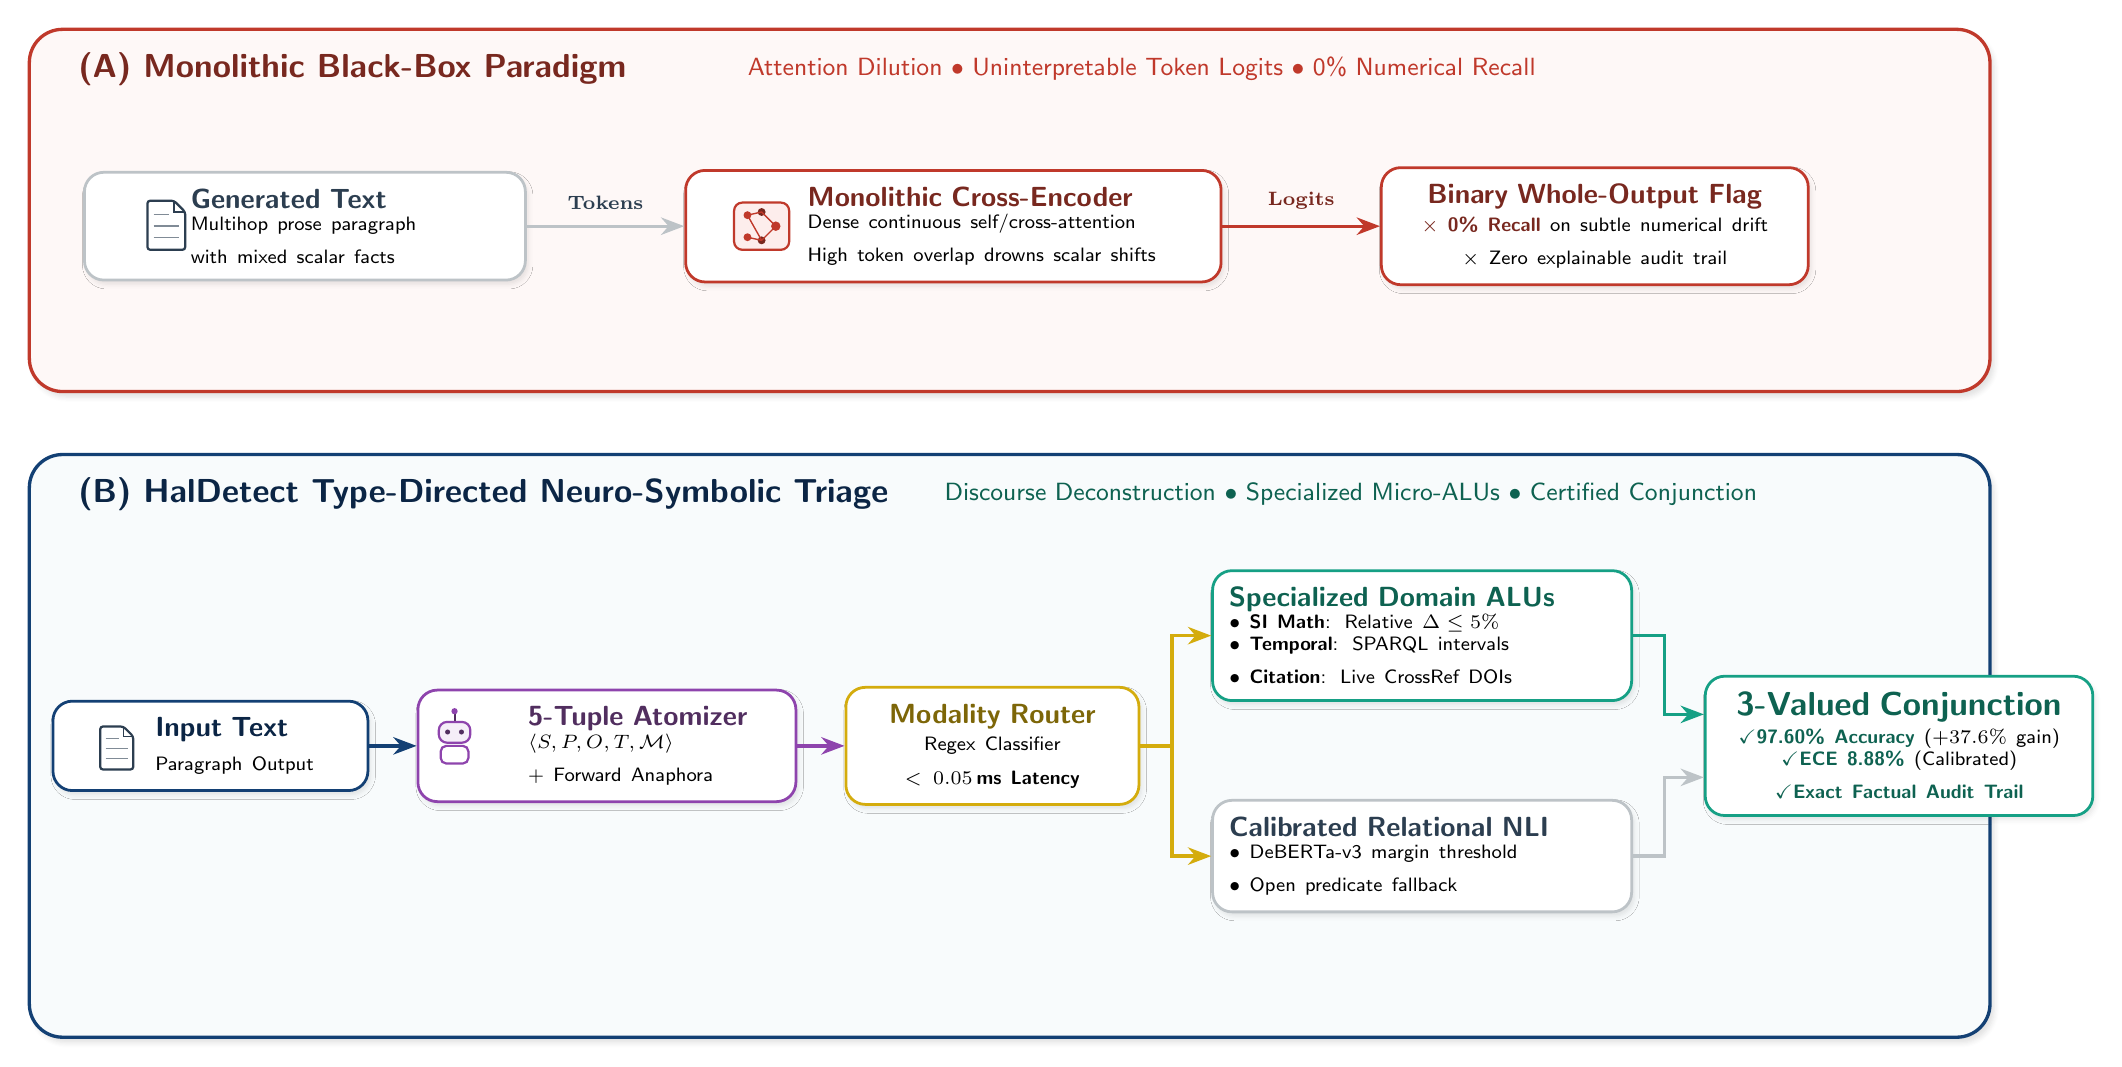
\begin{tikzpicture}[
    font=\sffamily,
    >=Stealth,
    trackbox/.style={
        draw=#1Border, fill=#1Light!40, line width=1.2pt, rounded corners=12pt,
        blur shadow={shadow blur steps=5, shadow xshift=1.5pt, shadow yshift=-2pt, shadow opacity=12}
    },
    card/.style={
        draw=#1Border, fill=white, line width=1.0pt, rounded corners=7pt,
        blur shadow={shadow blur steps=4, shadow xshift=1pt, shadow yshift=-1.5pt, shadow opacity=10},
        align=left, inner sep=6pt
    },
    wire/.style={
        ->, line width=1.2pt, draw=#1Border
    }
]

% Macro for doc
\newcommand{\drawDoc}[3]{%
    \begin{scope}[shift={(#1,#2)}, scale=#3]
        \draw[fill=white, draw=slateDark, line width=0.8pt, rounded corners=1pt] 
            (0,0) -- (0.6,0) -- (0.6,0.6) -- (0.42,0.78) -- (0,0.78) -- cycle;
        \draw[draw=slateDark, line width=0.6pt] (0.42,0.78) -- (0.42,0.6) -- (0.6,0.6);
        \draw[draw=slateDark!60, line width=0.5pt] (0.1,0.56) -- (0.35,0.56);
        \draw[draw=slateDark!60, line width=0.5pt] (0.1,0.38) -- (0.5,0.38);
        \draw[draw=slateDark!60, line width=0.5pt] (0.1,0.2) -- (0.5,0.2);
    \end{scope}
}

% Macro for Neural Brain
\newcommand{\drawBrain}[3]{%
    \begin{scope}[shift={(#1,#2)}, scale=#3]
        \draw[fill=crimsonLight, draw=crimsonBorder, line width=0.8pt, rounded corners=3pt] (-0.35,-0.3) rectangle (0.35,0.3);
        \fill[crimsonBorder] (-0.18,0.14) circle (0.05);
        \fill[crimsonBorder] (-0.18,-0.14) circle (0.05);
        \fill[crimsonDark] (0.0,0.18) circle (0.05);
        \fill[crimsonDark] (0.0,-0.18) circle (0.05);
        \fill[crimsonBorder] (0.18,0.0) circle (0.06);
        \draw[draw=crimsonBorder, line width=0.5pt] (-0.18,0.14) -- (0.0,0.18) -- (0.18,0.0);
        \draw[draw=crimsonBorder, line width=0.5pt] (-0.18,-0.14) -- (0.0,-0.18) -- (0.18,0.0);
        \draw[draw=crimsonBorder, line width=0.5pt] (-0.18,0.14) -- (0.0,-0.18);
    \end{scope}
}

% Macro for Robot
\newcommand{\drawMiniRobot}[3]{%
    \begin{scope}[shift={(#1,#2)}, scale=#3]
        \draw[line width=0.7pt, draw=purpleDark] (0, 0.35) -- (0, 0.52);
        \fill[purpleBorder] (0, 0.55) circle (0.05);
        \draw[fill=purpleLight, draw=purpleBorder, line width=0.8pt, rounded corners=3pt] (-0.25, 0.05) rectangle (0.25, 0.38);
        \fill[purpleDark] (-0.11, 0.22) circle (0.04);
        \fill[purpleDark] (0.11, 0.22) circle (0.04);
        \draw[fill=white, draw=purpleBorder, line width=0.8pt, rounded corners=2pt] (-0.22, -0.28) rectangle (0.22, 0.0);
    \end{scope}
}


% ==================== PARADIGM A: MONOLITHIC BLACK-BOX ====================
\draw[trackbox=crimson] (-0.5, 3.4) rectangle (24.4, 8.0);
\node[anchor=west, font=\sffamily\bfseries\large, text=crimsonDark] at (0.0, 7.5) {(A) Monolithic Black-Box Paradigm};
\node[anchor=west, font=\sffamily\small, text=crimsonBorder] at (8.5, 7.5) {Attention Dilution $\bullet$ Uninterpretable Token Logits $\bullet$ 0\% Numerical Recall};

\node[card=slate, minimum width=5.6cm, text width=4.5cm] (a_in) at (3.0, 5.5) {
    \hspace*{0.8cm}\textbf{\color{slateDark} Generated Text}\\
    \hspace*{0.8cm}\scriptsize Multihop prose paragraph\\
    \hspace*{0.8cm}\scriptsize with mixed scalar facts
};
\drawDoc{1.0}{5.2}{0.8}

\node[card=crimson, right=2.0cm of a_in, minimum width=6.8cm, text width=5.5cm] (a_enc) {
    \hspace*{0.9cm}\textbf{\color{crimsonDark} Monolithic Cross-Encoder}\\
    \hspace*{0.9cm}\scriptsize Dense continuous self/cross-attention\\
    \hspace*{0.9cm}\scriptsize High token overlap drowns scalar shifts
};
\drawBrain{8.8}{5.5}{1.0}

\node[card=crimson, right=2.0cm of a_enc, minimum width=5.4cm, text width=5.0cm, align=center] (a_out) {
    \textbf{\color{crimsonDark} Binary Whole-Output Flag}\\
    \vspace{2pt}
    \scriptsize \textbf{\color{crimsonDark}$\times$ 0\% Recall} on subtle numerical drift\\
    \scriptsize $\times$ Zero explainable audit trail
};

\draw[wire=slate] (a_in) -- (a_enc) node[midway, above=2pt, font=\scriptsize\bfseries, text=slateDark] {Tokens};
\draw[wire=crimson] (a_enc) -- (a_out) node[midway, above=2pt, font=\scriptsize\bfseries, text=crimsonDark] {Logits};


% ==================== PARADIGM B: HALDETECT NEURO-SYMBOLIC ====================
\draw[trackbox=navy] (-0.5, -4.8) rectangle (24.4, 2.6);
\node[anchor=west, font=\sffamily\bfseries\large, text=navyDark] at (0.0, 2.1) {(B) HalDetect Type-Directed Neuro-Symbolic Triage};
\node[anchor=west, font=\sffamily\small, text=emeraldDark] at (11.0, 2.1) {Discourse Deconstruction $\bullet$ Specialized Micro-ALUs $\bullet$ Certified Conjunction};

\node[card=navy, minimum width=4.0cm, text width=2.8cm] (b_in) at (1.8, -1.1) {
    \hspace*{0.7cm}\textbf{\color{navyDark} Input Text}\\
    \hspace*{0.7cm}\scriptsize Paragraph Output
};
\drawDoc{0.4}{-1.4}{0.7}

\node[card=purple, right=0.6cm of b_in, minimum width=4.8cm, text width=3.6cm] (b_atom) {
    \hspace*{0.8cm}\textbf{\color{purpleDark} 5-Tuple Atomizer}\\
    \hspace*{0.8cm}\scriptsize $\langle S, P, O, T, \mathcal{M} \rangle$\\
    \hspace*{0.8cm}\scriptsize + Forward Anaphora
};
\drawMiniRobot{4.9}{-1.1}{0.8}

\node[card=amber, right=0.6cm of b_atom, minimum width=3.6cm, text width=3.3cm, align=center] (b_router) {
    \textbf{\color{amberDark} Modality Router}\\
    \vspace{2pt}
    \scriptsize Regex Classifier\\
    \scriptsize \textbf{$<0.05\,\text{ms}$ Latency}
};

% ALU Stack
\node[card=emerald, anchor=west, minimum width=5.2cm, text width=4.9cm, align=left] (b_alu) at ($(b_router.east) + (0.9cm, 1.4cm)$) {
    \textbf{\color{emeraldDark} Specialized Domain ALUs}\\
    \scriptsize $\bullet$ \textbf{SI Math}: Relative $\Delta \le 5\%$\\
    \scriptsize $\bullet$ \textbf{Temporal}: SPARQL intervals\\
    \scriptsize $\bullet$ \textbf{Citation}: Live CrossRef DOIs
};

\node[card=slate, anchor=west, minimum width=5.2cm, text width=4.9cm, align=left] (b_nli) at ($(b_router.east) + (0.9cm, -1.4cm)$) {
    \textbf{\color{slateDark} Calibrated Relational NLI}\\
    \scriptsize $\bullet$ DeBERTa-v3 margin threshold\\
    \scriptsize $\bullet$ Open predicate fallback
};

% Output Conjunction
\node[card=emerald, right=0.9cm of $(b_alu.east)!0.5!(b_nli.east)$, minimum width=4.8cm, text width=4.5cm, align=center] (b_decision) {
    \textbf{\color{emeraldDark}\large 3-Valued Conjunction}\\
    \vspace{2pt}
    \scriptsize \textbf{\color{emeraldDark}\checkmark 97.60\% Accuracy} ($+37.6\%$ gain)\\
    \scriptsize \textbf{\color{emeraldDark}\checkmark ECE 8.88\%} (Calibrated)\\
    \scriptsize \textbf{\color{emeraldDark}\checkmark Exact Factual Audit Trail}
};

% Wires
\draw[wire=navy] (b_in) -- (b_atom);
\draw[wire=purple] (b_atom) -- (b_router);
\draw[wire=amber] (b_router.east) -- ++(0.4,0) |- (b_alu.west);
\draw[wire=amber] (b_router.east) -- ++(0.4,0) |- (b_nli.west);

\draw[wire=emerald] (b_alu.east) -| ++(0.4,-0.6) |- ($(b_decision.west) + (0, 0.4)$);
\draw[wire=slate] (b_nli.east) -| ++(0.4,0.6) |- ($(b_decision.west) + (0, -0.4)$);

\end{tikzpicture}
\end{document}
